%%%%%%%%%%%%%%%%%%%%%%%%%%%%%%%%%%%%%%%%%
% Beamer Presentation
% LaTeX Template
% Version 1.0 (10/11/12)
%
% This template has been downloaded from:
% http://www.LaTeXTemplates.com
%
% License:
% CC BY-NC-SA 3.0 (http://creativecommons.org/licenses/by-nc-sa/3.0/)
%
%%%%%%%%%%%%%%%%%%%%%%%%%%%%%%%%%%%%%%%%%

%----------------------------------------------------------------------------------------
%	PACKAGES AND THEMES
%----------------------------------------------------------------------------------------

\documentclass{beamer}

\mode<presentation> {

% The Beamer class comes with a number of default slide themes
% which change the colors and layouts of slides. Below this is a list
% of all the themes, uncomment each in turn to see what they look like.

%\usetheme{default}
%\usetheme{AnnArbor}
%\usetheme{Antibes}
%\usetheme{Bergen}
%\usetheme{Berkeley}
%\usetheme{Berlin}
\usetheme{Boadilla}
%\usetheme{CambridgeUS}
%\usetheme{Copenhagen}
%\usetheme{Darmstadt}
%\usetheme{Dresden}
%\usetheme{Frankfurt}
%\usetheme{Goettingen}
%\usetheme{Hannover}
%\usetheme{Ilmenau}
%\usetheme{JuanLesPins}
%\usetheme{Luebeck}
%\usetheme{Madrid}
%\usetheme{Malmoe}
%\usetheme{Marburg}
%\usetheme{Montpellier}
%\usetheme{PaloAlto}
%\usetheme{Pittsburgh}
%\usetheme{Rochester}
%\usetheme{Singapore}
%\usetheme{Szeged}
%\usetheme{Warsaw}

% As well as themes, the Beamer class has a number of color themes
% for any slide theme. Uncomment each of these in turn to see how it
% changes the colors of your current slide theme.

%\usecolortheme{albatross}
%\usecolortheme{beaver}
%\usecolortheme{beetle}
%\usecolortheme{crane}
%\usecolortheme{dolphin}
%\usecolortheme{dove}
%\usecolortheme{fly}
%\usecolortheme{lily}
%\usecolortheme{orchid}
%\usecolortheme{rose}
%\usecolortheme{seagull}
%\usecolortheme{seahorse}
%\usecolortheme{whale}
%\usecolortheme{wolverine}

\usepackage[official]{eurosym}
\usepackage{svg}
\usepackage{amsmath}
\usepackage{graphicx}
\usepackage{multirow}
\usepackage[utf8]{inputenc}
%\setbeamertemplate{footline} % To remove the footer line in all slides uncomment this line
%\setbeamertemplate{footline}[page number] % To replace the footer line in all slides with a simple slide count uncomment this line

%\setbeamertemplate{navigation symbols}{} % To remove the navigation symbols from the bottom of all slides uncomment this line
}

\usepackage{graphicx} % Allows including images
\usepackage{booktabs} % Allows the use of \toprule, \midrule and \bottomrule in tables

%----------------------------------------------------------------------------------------
%	TITLE PAGE
%----------------------------------------------------------------------------------------

\title[Revenue Maximisation]{Revenue maximisation by intelligent couponing} % The short title appears at the bottom of every slide, the full title is only on the title page

\author{Thomas Friedrich, Lukas Schmauch}
 % Your name
\institute[FSU] % Your institution as it will appear on the bottom of every slide, may be shorthand to save space
{
Friedrich-Schiller-Universität Jena \\ % Your institution for the title page
}
\date{20. Januar 2020} % Date, can be changed to a custom date

\begin{document}
\begin{frame}
\titlepage % Print the title page as the first slide
\end{frame}
%-------------------------------------
\begin{frame}
\frametitle{Übersicht} 
\tableofcontents
\section{Aufgabenstellung und Datensatz} 
\section{Klassifikation und Evaluation} 
\end{frame}

%----------------------------------------------------------------------------------------
%	PRESENTATION SLIDES
%----------------------------------------------------------------------------------------
\begin{frame}

\frametitle{Ausgangssituation}
\begin{itemize}
	\item Data Mining Cup 2010
	\item \textbf{Ziel:} Gewinnmaximierung anhand der Ermittlung der Wiederkäufer
\end{itemize}
\begin{table}[h]
\small
\begin{tabular}{c r|c|c|}
            & & \multicolumn{2}{c|}{Vorhergesagt}             \\
            &	&kein Wiederkäufer(0)   &Wiederkäufer(1)            \\ \hline
            \multirow{2}*{Tatsächlich} &kein Wiederkäufer(0)&1.5   &0               \\
            &Wiederkäufer(1)&-5   &0              \\ \hline
      \end{tabular}
      %\caption{Kostenmatrix}
\end{table}


\end{frame}
%---------------------------------------
\begin{frame}
\frametitle{Der Datensatz}
\begin{columns}[c] % The "c" option specifies centered vertical alignment while the "t" option is used for top vertical alignment

\column{.3\textwidth} % Left column and width
\begin{footnotesize}
\begin{itemize}
\item 64854 Einträge
\item 50:50 Train/ Test 
\item 38 Merkmale
\item 20 numerisch
\item 18 kategorisch
\end{itemize}
\end{footnotesize}

\column{.5\textwidth} % Right column and width
\begin{figure}
\begin{center}
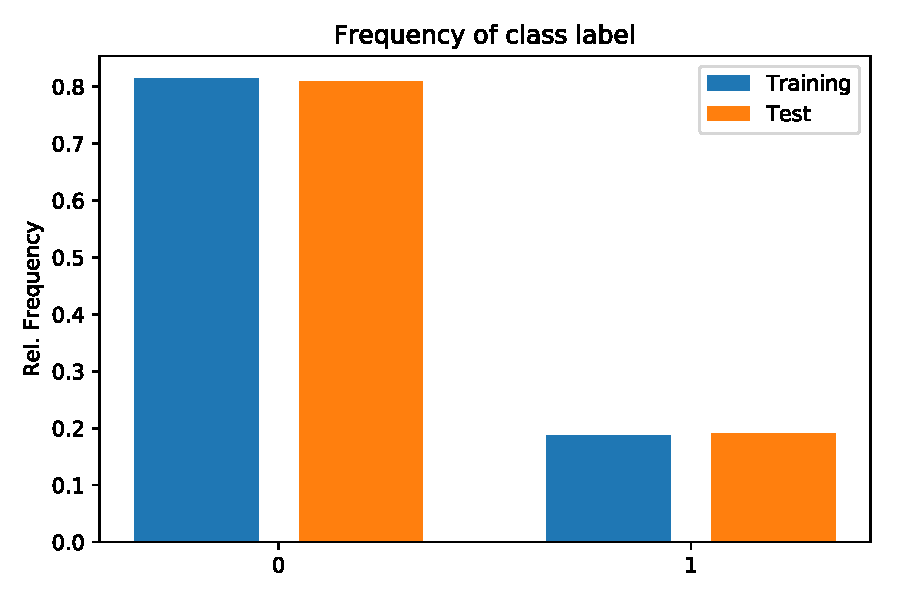
\includegraphics[width=1.0\textwidth]{pdf/distTrainTest.pdf}
\end{center}
%\caption{Verteilung Klassenlabel}
\end{figure}
\end{columns}
\end{frame}

%---------------------------------------

\begin{frame}
\begin{footnotesize}
\begin{itemize}
\item  \textbf{erzielter Umsatz:} 8552.00 \euro{}
\item \textbf{Umsatzsteigerung:}	0.04093 \% 
\item \textbf{Accuracy:} 81.00 \%
\end{itemize}
\end{footnotesize}

\frametitle{Konfusionsmatrix Naiver Run (Decision Tree)}
\begin{figure}
\begin{center}
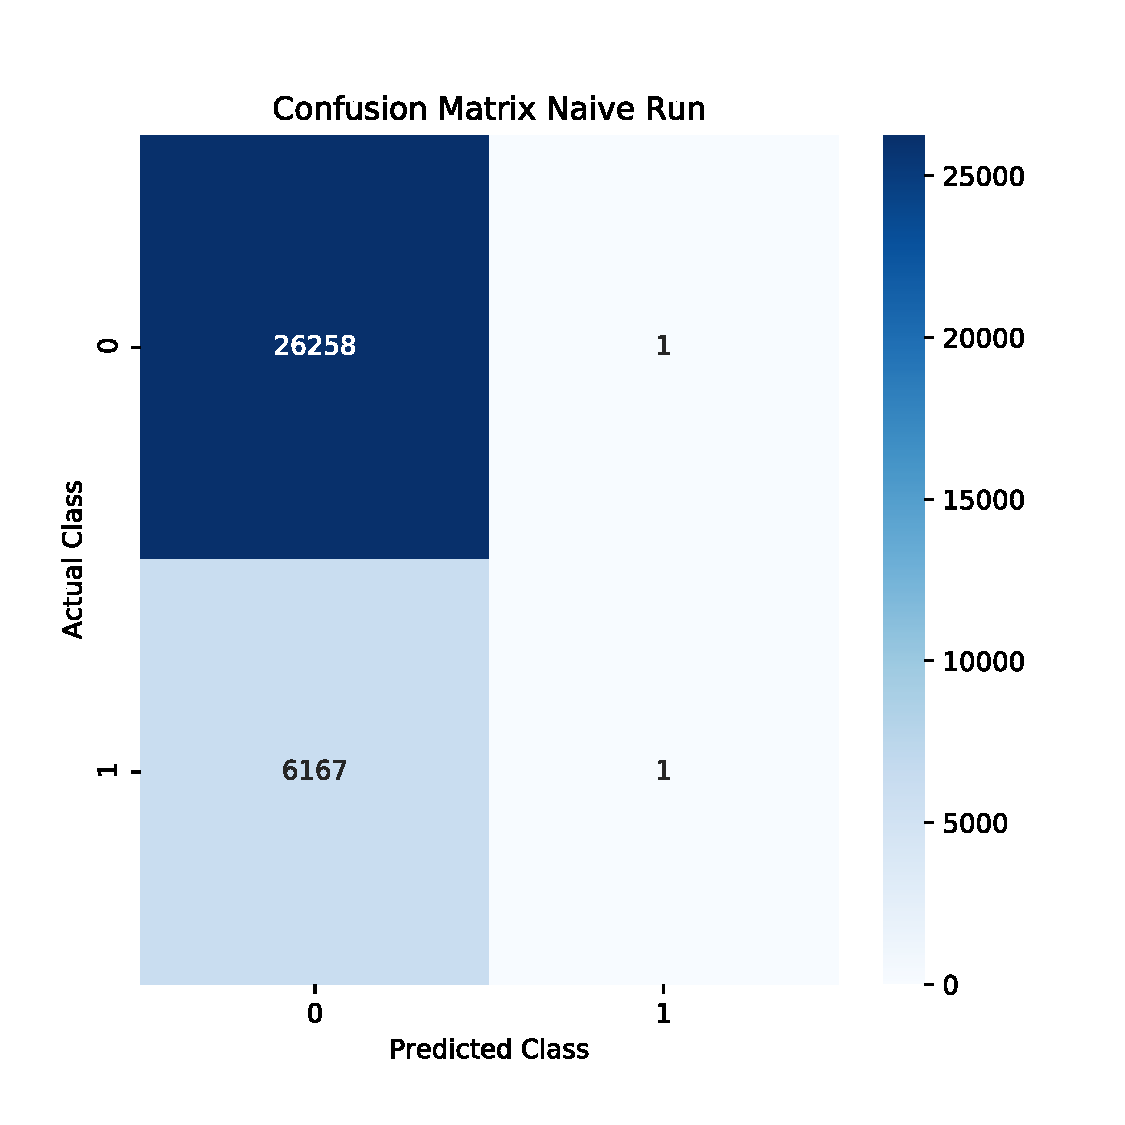
\includegraphics[width=.5\textwidth]{pdf/confusion1.pdf}
\end{center}
%\caption{Konfusionsmatrix Naiver Run}
\end{figure}
\end{frame}

%------------------------------------------------
%\begin{frame}
%\frametitle{Oversampling}
%\begin{center}
%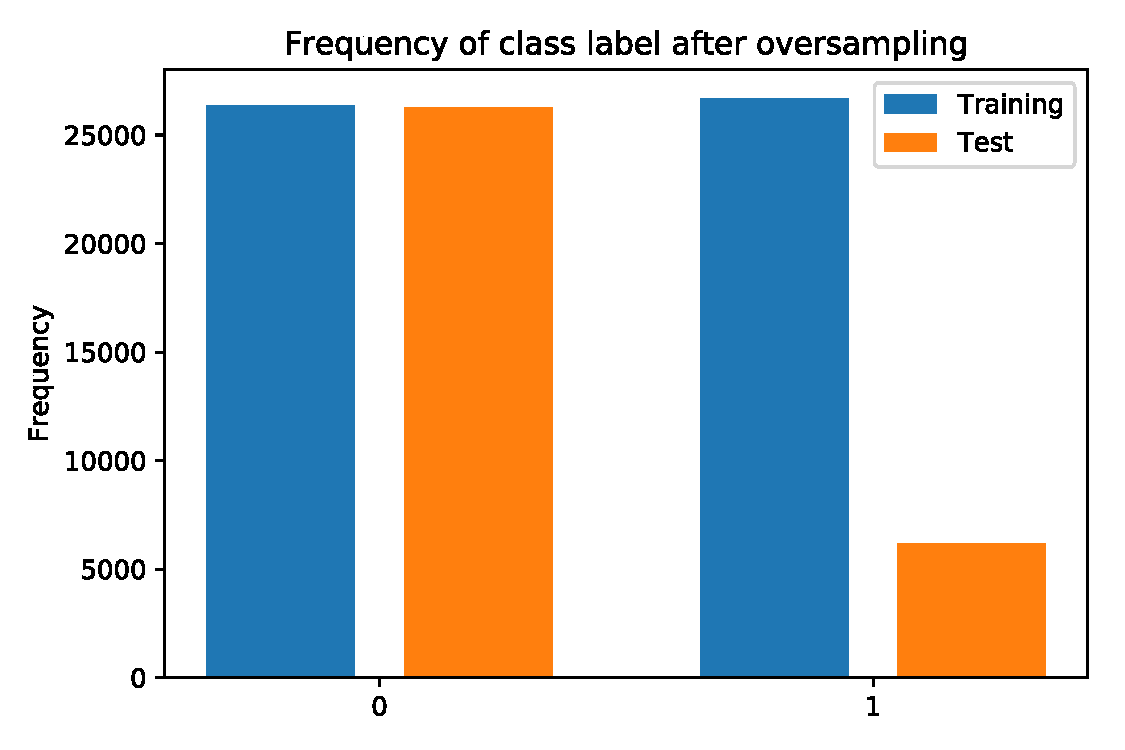
\includegraphics[width=0.7\textwidth]{pdf/oversampled.pdf}
%\end{center}
%\end{frame}
%------------------------------------------------
\begin{frame}
\frametitle{Konfusionsmatrix nach Oversampling (Decision Tree)}
\begin{columns}[c] % The "c" option specifies centered vertical alignment while the "t" option is used for top vertical alignment

\column{.5\textwidth} % Left column and width
\begin{tiny}
\begin{itemize}
\item  \textbf{erzielter Umsatz:} 11520.00 \euro{}
\item \textbf{Umsatzsteigerung:}	25.79 \% 
\item \textbf{Accuracy:} 75.23 \%
\end{itemize}
\end{tiny}

\begin{figure}
\begin{center}
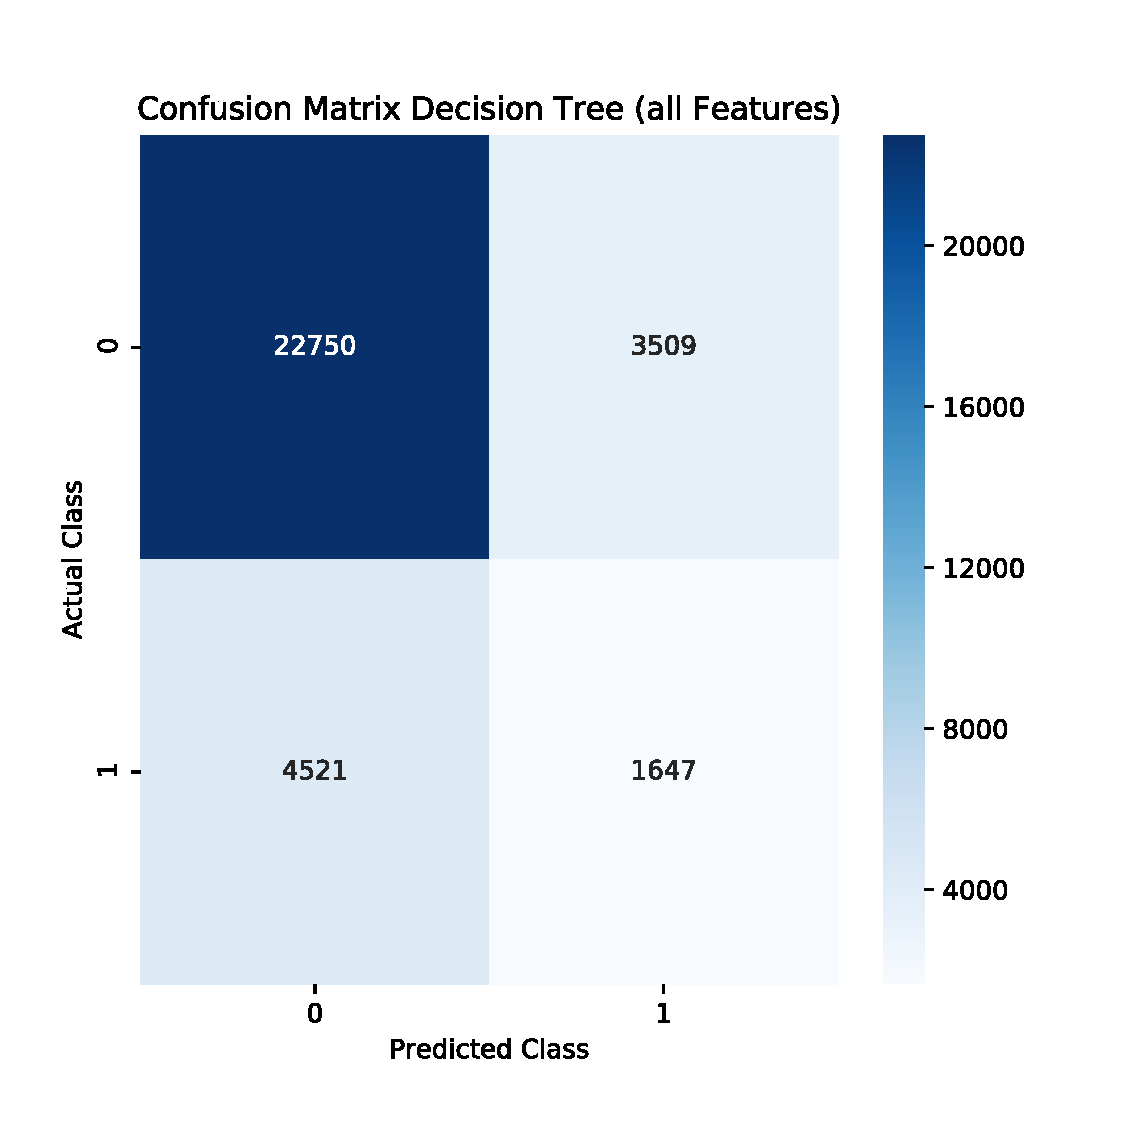
\includegraphics[width=.8\textwidth]{pdf/confusion2.pdf}
\end{center}
%\caption{Konfusionsmatrix nach Oversampling}
\end{figure}


\column{.5\textwidth} % Right column and width
\begin{center}
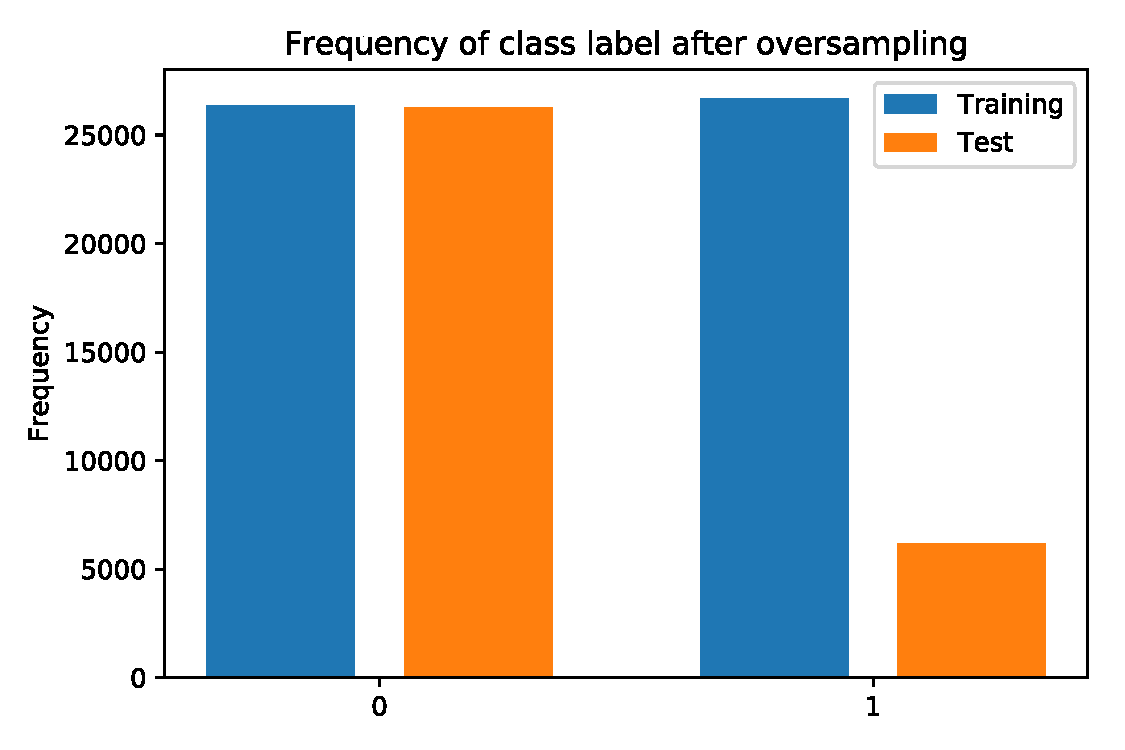
\includegraphics[width=.8\textwidth]{pdf/oversampled.pdf}
\end{center}
\end{columns}
\end{frame}


%------------------------------------------------

%\begin{frame}
%\frametitle{Konfusionsmatrix nach Oversampling (Decision Tree)}
%\begin{footnotesize}
%\begin{itemize}
%\item  \textbf{erzielter Umsatz:} 11520.00 \euro{}
%\item \textbf{Umsatzsteigerung:}	25.79 \% 
%\item \textbf{Accuracy:} 75.23 \%
%\end{itemize}
%\end{footnotesize}
%
%\begin{figure}
%\begin{center}
%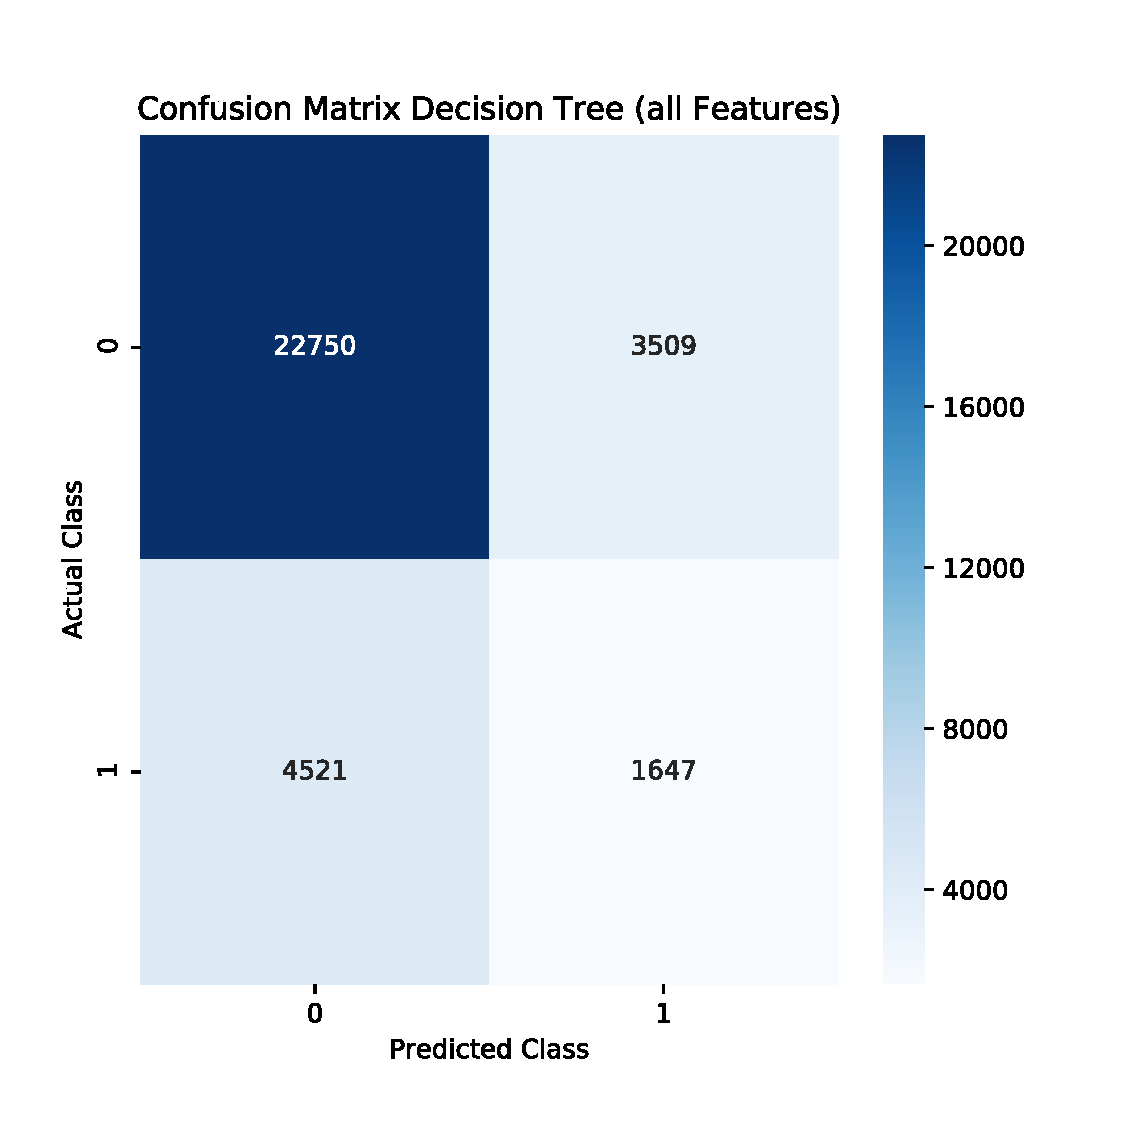
\includegraphics[width=.5\textwidth]{pdf/confusion2.pdf}
%\end{center}
%%\caption{Konfusionsmatrix nach Oversampling}
%\end{figure}
%\end{frame}
%------------------------------------------------
\begin{frame}
\frametitle{Backward Feature Elimination}
\begin{figure}
\begin{center}
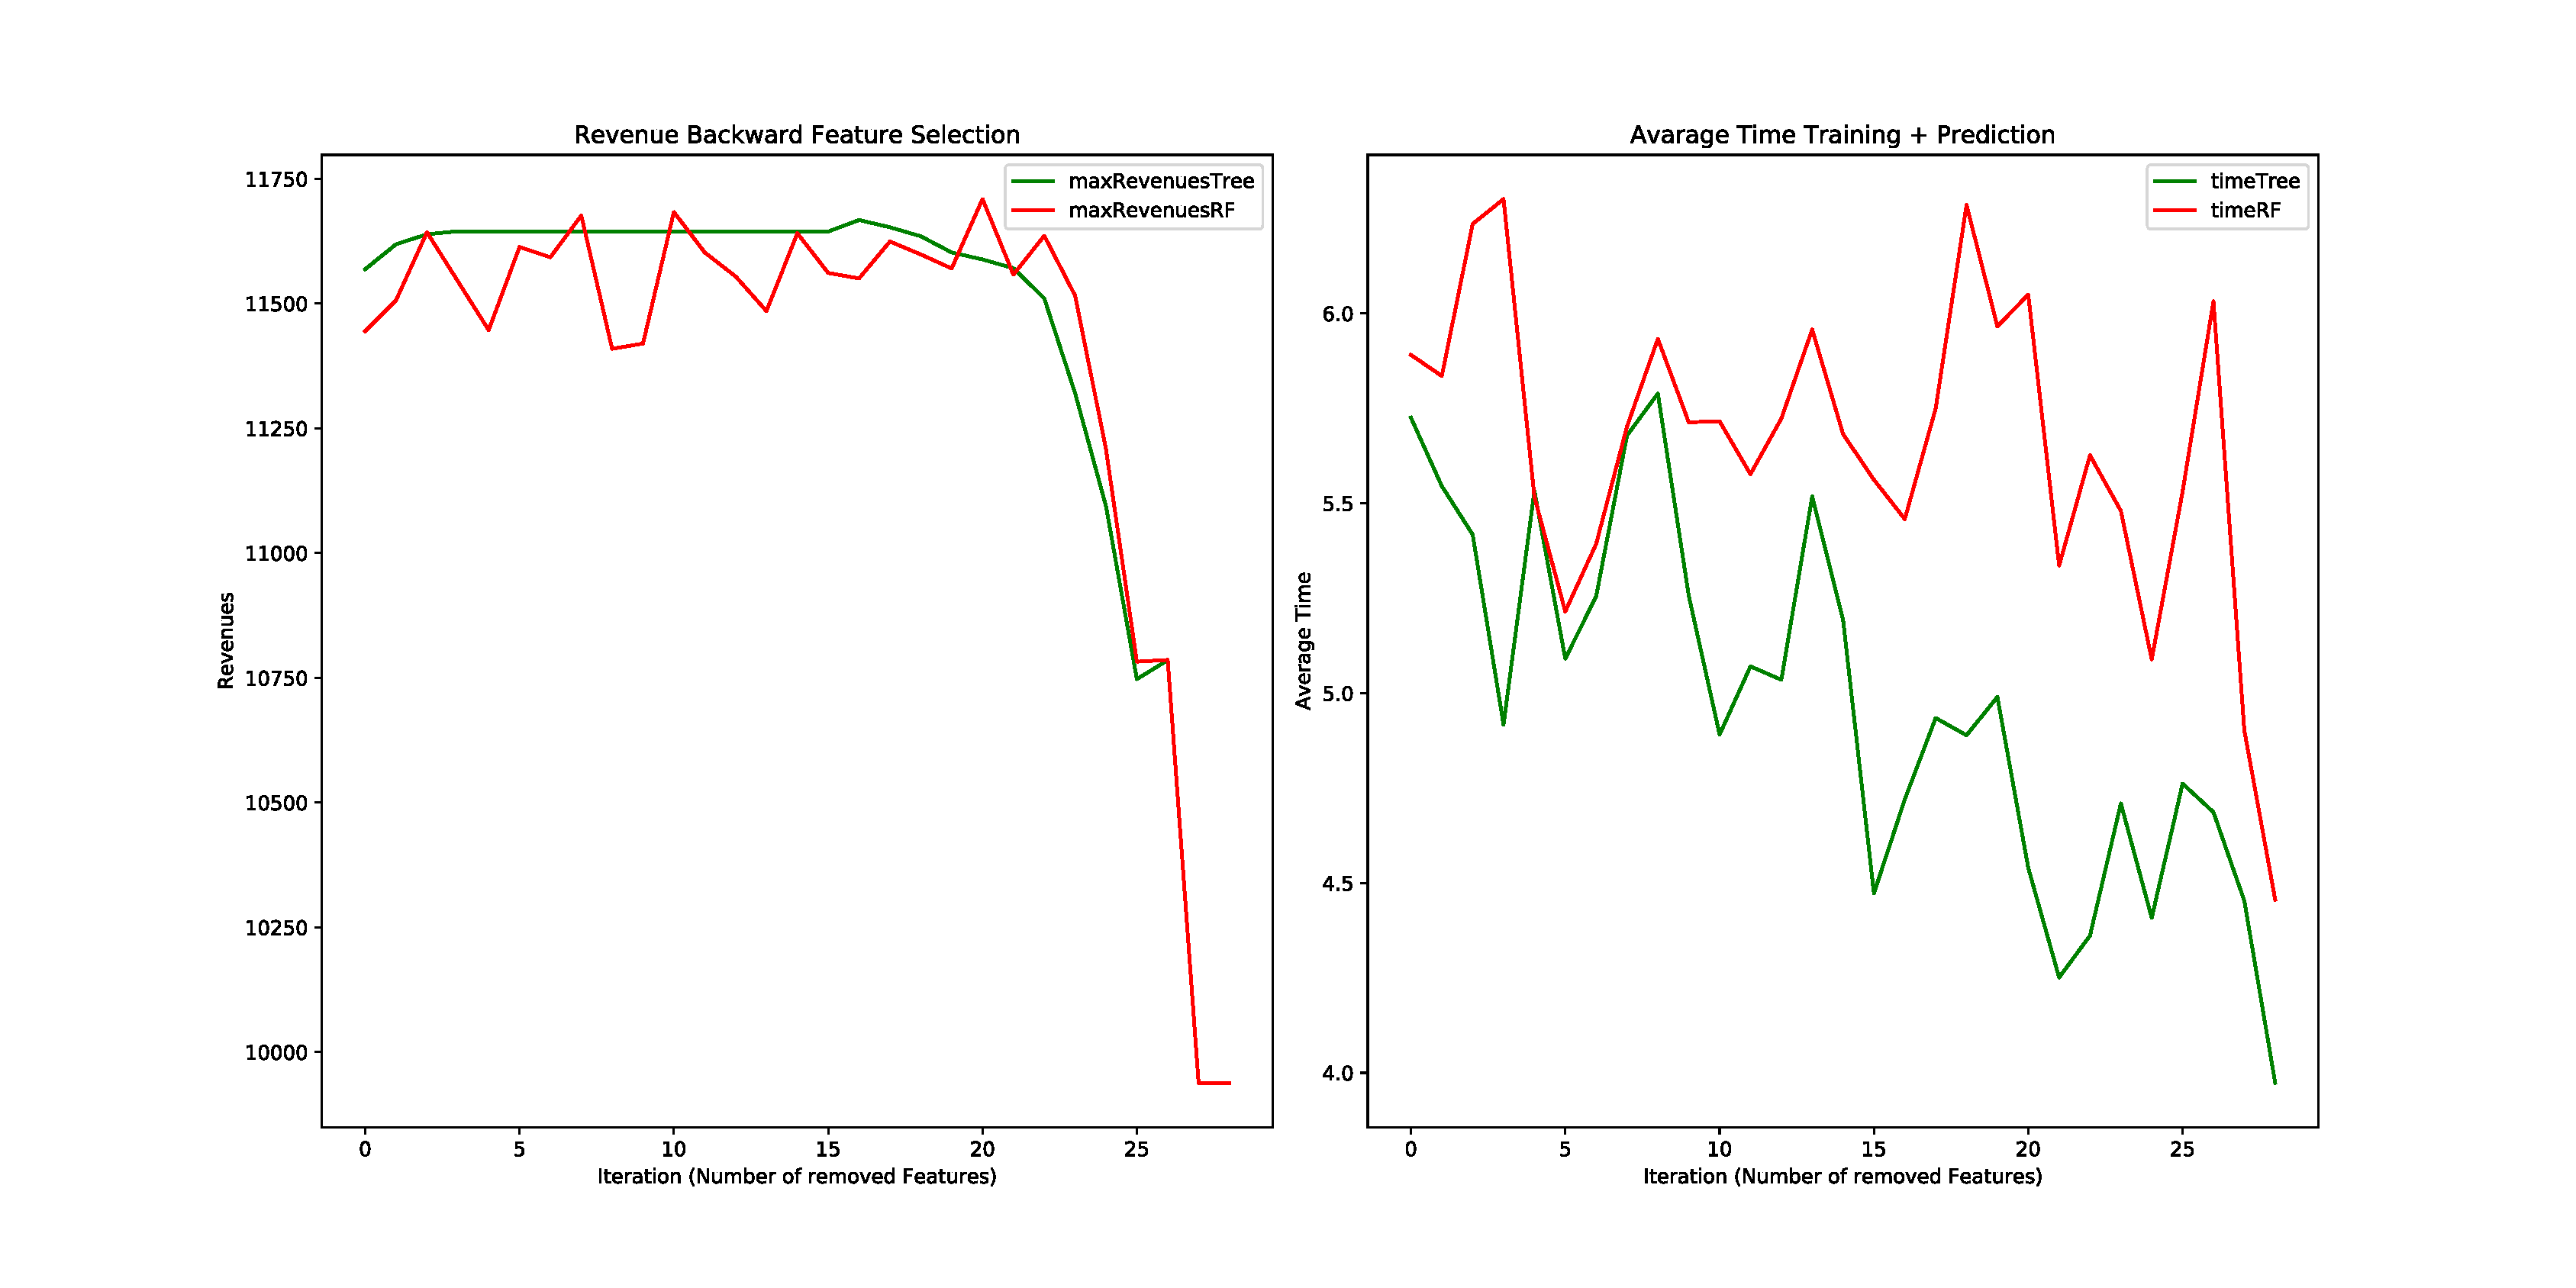
\includegraphics[width=1.0\textwidth]{pdf/backwardSpark.pdf}
\end{center}
%\caption{Konfusionsmatrix Naiver Run}
\end{figure}
\end{frame}

%------------------------------------------------
\begin{frame}
\frametitle{Zusammenfassung der Ergebnisse}
\begin{table}
\begin{tabular}{l c c}
\toprule
\textbf{Klassifikator} & \textbf{Umsatz} & \textbf{Steigerung}\\
\midrule
Ohne Optimierung & 8548.50 \euro{} & - \\
Decision Tree Naiv & 8552.00 \euro{} & 0.0004 \%\\
Decision Tree Oversampling  & 11667.50 \euro{} & 36.4859 \% \\
Random Forest Oversampling  & 11709.50 \euro{} &  36.9772 \% \\
Optimaler Klassifikator  & 39388.50 \euro{} &  -\\
\bottomrule
\end{tabular}
%\caption{Ergebnisse}
\end{table}
\end{frame}


%------------------------------------------------

\begin{frame}
\frametitle{Quelle: Aufgabenstellung und Datensatz}
\footnotesize{
\begin{thebibliography}{99} % Beamer does not support BibTeX so references must be inserted manually as below
\bibitem[DMC, 2010]{p1} Data Mining Cup 2010
\newblock https://www.data-mining-cup.com/reviews/dmc-2010/
\end{thebibliography}
}
\end{frame}

%------------------------------------------------



%----------------------------------------------------------------------------------------

\end{document} 